% arara: pdflatex: { shell: yes }
\documentclass{article}
\usepackage[utf8]{inputenc}
\usepackage{array}
\usepackage{hyperref}
\usepackage{float}
\usepackage{graphicx}
\bibliographystyle{apacite}

% Suppress underfull and overfull warnings
\hbadness=10000
\hfuzz=10000pt

\begin{document}

\title{Object-relational database}
\author{Erick Gonzalez Parada 178145\\
    Antonio Gutiérrez Blanco 177442\\
    Andre Francois Duhamel Gutierrez 177315\\
    Emiliano Ruiz Plancarte 177478\\ }
\date{\today}

\maketitle

\section{Objective}
\begin{sloppypar}
To design, implement, and evaluate an object-relational database system by defining complex object types, creating relational tables with nested collections, and establishing relationships between objects. The goal is to demonstrate the effective use of Object Query Language (OQL) for managing object-relational data structures, inserting sample data, and performing queries to validate the schema's functionality and integrity.
\end{sloppypar}

\section{Introduction}

\vspace{1cm}

{\Huge{ There is an EXTRA section at the end\\ please don't forget}}

\vspace{1cm}
Object Query Language (OQL) is a standardized query language designed for querying and manipulating object-oriented databases. Unlike traditional SQL, which is tailored for relational databases, OQL is specifically built to handle complex object-oriented data structures, such as inheritance, polymorphism, and nested collections. OQL allows developers to interact with object-relational databases in a way that aligns with the principles of object-oriented programming, making it a powerful tool for modern database systems\cite{ibm}.
\\
OQL revolves around its ability to query objects and their relationships directly, rather than relying on flat, tabular structures. This is particularly useful in scenarios where data is represented as objects with attributes, methods, and relationships to other objects\cite{mendix}.

\section{Literature Review}

Traditional SQL (Structured Query Language) is designed for relational databases, where data is stored in flat, tabular structures. The philosophy of SQL revolves around the use of \textbf{joins} to combine data from multiple tables, enabling users to retrieve related information. For example, to retrieve data about an employee and their department, SQL requires joining the \texttt{Employee} and \texttt{Department} tables using a common key. While this approach is effective for relational data, it becomes cumbersome and inefficient when dealing with complex, hierarchical, or object-oriented data structures\cite{w3s}.

In contrast, Object Query Language (OQL) is specifically designed for object-oriented databases, where data is represented as objects with attributes, methods, and relationships. OQL eliminates the need for explicit joins by allowing developers to \textbf{directly traverse object relationships}. For instance, in an object-relational database, an \texttt{Employee} object might have a direct reference to a \texttt{Department} object. With OQL, querying the department of an employee is as simple as navigating the object hierarchy (e.g., \texttt{employee.department}), without the need for complex joins or intermediate tables\cite{mendix}.

While SQL can simulate some object-oriented behavior---such as using foreign keys and nested queries to represent relationships---it lacks the native support for object-oriented principles like \textbf{inheritance}, \textbf{polymorphism}, and \textbf{nested collections}. For example, simulating inheritance in SQL requires creating multiple tables and using complex joins to represent parent-child relationships. Similarly, representing nested collections (e.g., a list of phone numbers for an employee) often involves creating additional tables and performing multiple joins, which can lead to inefficient queries and increased complexity\cite{ibm}.

OQL, on the other hand, natively supports these object-oriented features. It allows developers to define \textbf{complex object types}, \textbf{inheritance hierarchies}, and \textbf{nested collections} directly in the database schema. This makes OQL more intuitive and efficient for querying object-oriented data, as it aligns with the natural structure of the data. For example, querying a nested collection of phone numbers in OQL is straightforward (e.g., \texttt{employee.phones}), whereas in SQL, it requires joining multiple tables and aggregating results\cite{mendix}.

In summary, while SQL remains a powerful tool for relational data, its reliance on joins and lack of native support for object-oriented principles make it less suitable for modern, object-oriented applications. OQL addresses these limitations by providing a query language that is inherently designed for object-relational databases, enabling more efficient and intuitive data retrieval and manipulation.

\section{Methodology}
To implement and evaluate the object-relational database system, we used \textbf{Oracle Database Express Edition (XE)} as the primary database management system. The general solution involved the following steps:

1. \textbf{Setting Up Oracle Database Express}:
   - Oracle Database XE was downloaded and installed on a local machine. During installation, the default settings were used, and a system password was set for the administrative user (\texttt{SYS}).
   - The database was configured to allow remote connections, and the necessary ports (e.g., 1521 for Oracle) were opened to enable access from external tools.

2. \textbf{Configuring Visual Studio Code (VSCode)}:
   - The \textbf{Oracle Developer Tools for VSCode} extension was installed to facilitate database connectivity and query execution.
   - A connection profile was created in VSCode, specifying the host (e.g., \texttt{localhost}), port (e.g., \texttt{1521}), service name (e.g., \texttt{XE}), and credentials (e.g., \texttt{SYS} and the system password).

	 \begin{figure}[H]
		 \centering
		 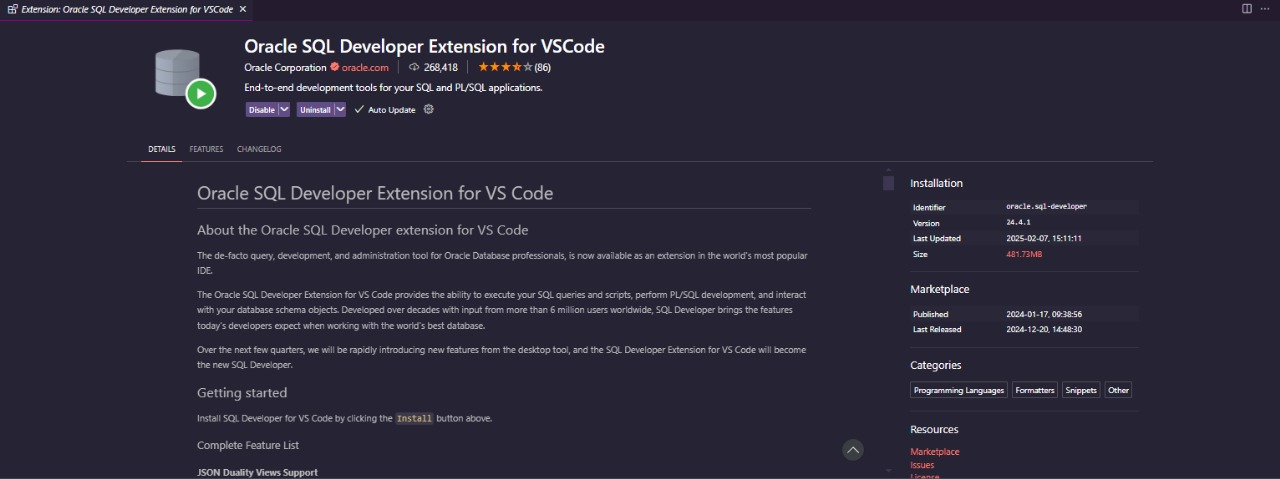
\includegraphics[width=1\textwidth]{imgs/ext.jpeg}
		 \caption{VSCode extension}
		 \label{fig:1}
		\end{figure}

3. \textbf{Writing and Executing OQL Scripts}:
   - OQL scripts were written to define complex object types, create relational tables with nested collections, and establish relationships between objects. These scripts were saved as \texttt{.sql} files for execution.
   - The scripts included:
     - \textbf{Object Type Definitions}: Creating object types such as \texttt{employee\_t}, \texttt{worker\_t}, and \texttt{manager\_t} with attributes and methods.
     - \textbf{Table Creation}: Defining tables with nested collections (e.g., \texttt{telephone\_t} as a nested table of phone numbers).
     - \textbf{Data Insertion}: Inserting sample data into the tables to populate the database.
     - \textbf{Query Execution}: Writing and executing queries to retrieve and validate data from the object-relational schema.

4. \textbf{Challenges Faced}:
   - One of the major challenges was the \textbf{lack of comprehensive online documentation} for OQL, especially in the context of Oracle Database. This made it difficult to troubleshoot issues and find examples of advanced OQL features.
   - Additionally, configuring the Oracle extension in VSCode required trial and error, as some settings (e.g., connection parameters) were not well-documented.

5. \textbf{Validation and Testing}:
   - After executing the OQL scripts, the database schema and data were validated by running queries to ensure that object relationships, nested collections, and inheritance hierarchies were functioning as expected.
   - The results were compared with the expected outcomes to verify the correctness and efficiency of the implemented schema.

\section{Result Analysis}
The following figures will show us the whole work done for our solution and how the oql compiled successfully:

\begin{figure}[H]
	\centering
	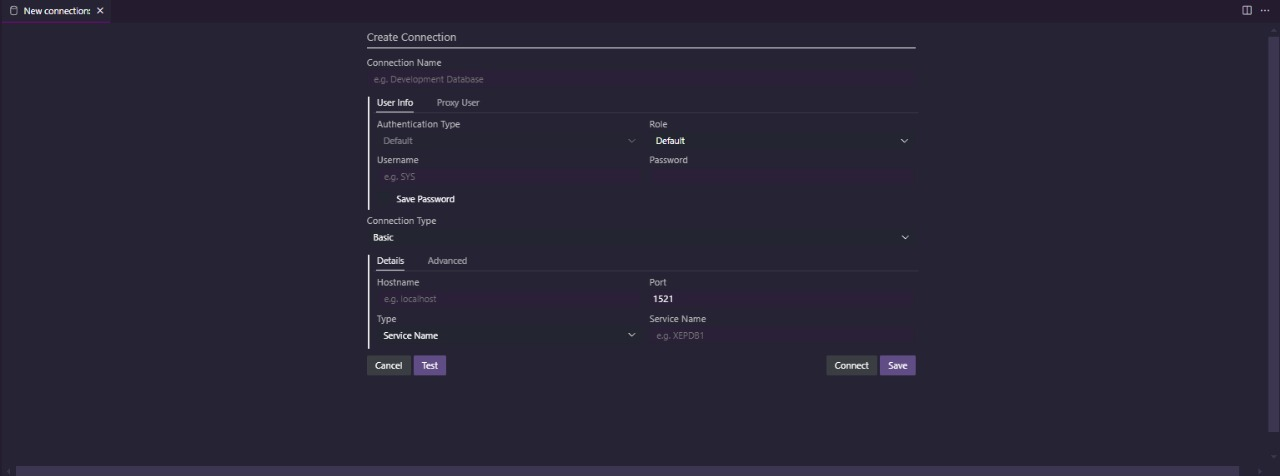
\includegraphics[width=1\textwidth]{imgs/cconn.jpeg}
	\caption{Create connection}
	\label{fig:2}
\end{figure}

\begin{figure}[H]
	\centering
	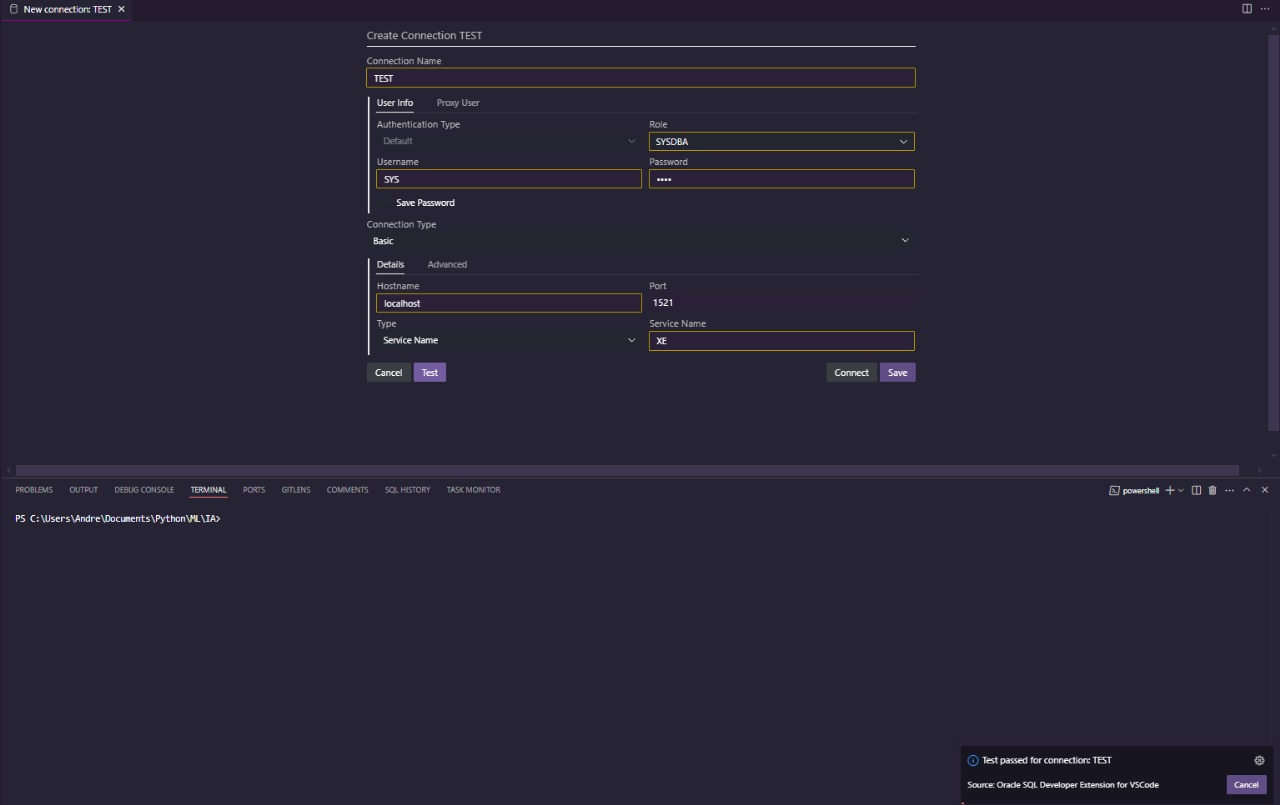
\includegraphics[width=1\textwidth]{imgs/setConn.jpeg}
	\caption{Setting connection}
	\label{fig:3}
\end{figure}

\begin{figure}[H]
	\centering
	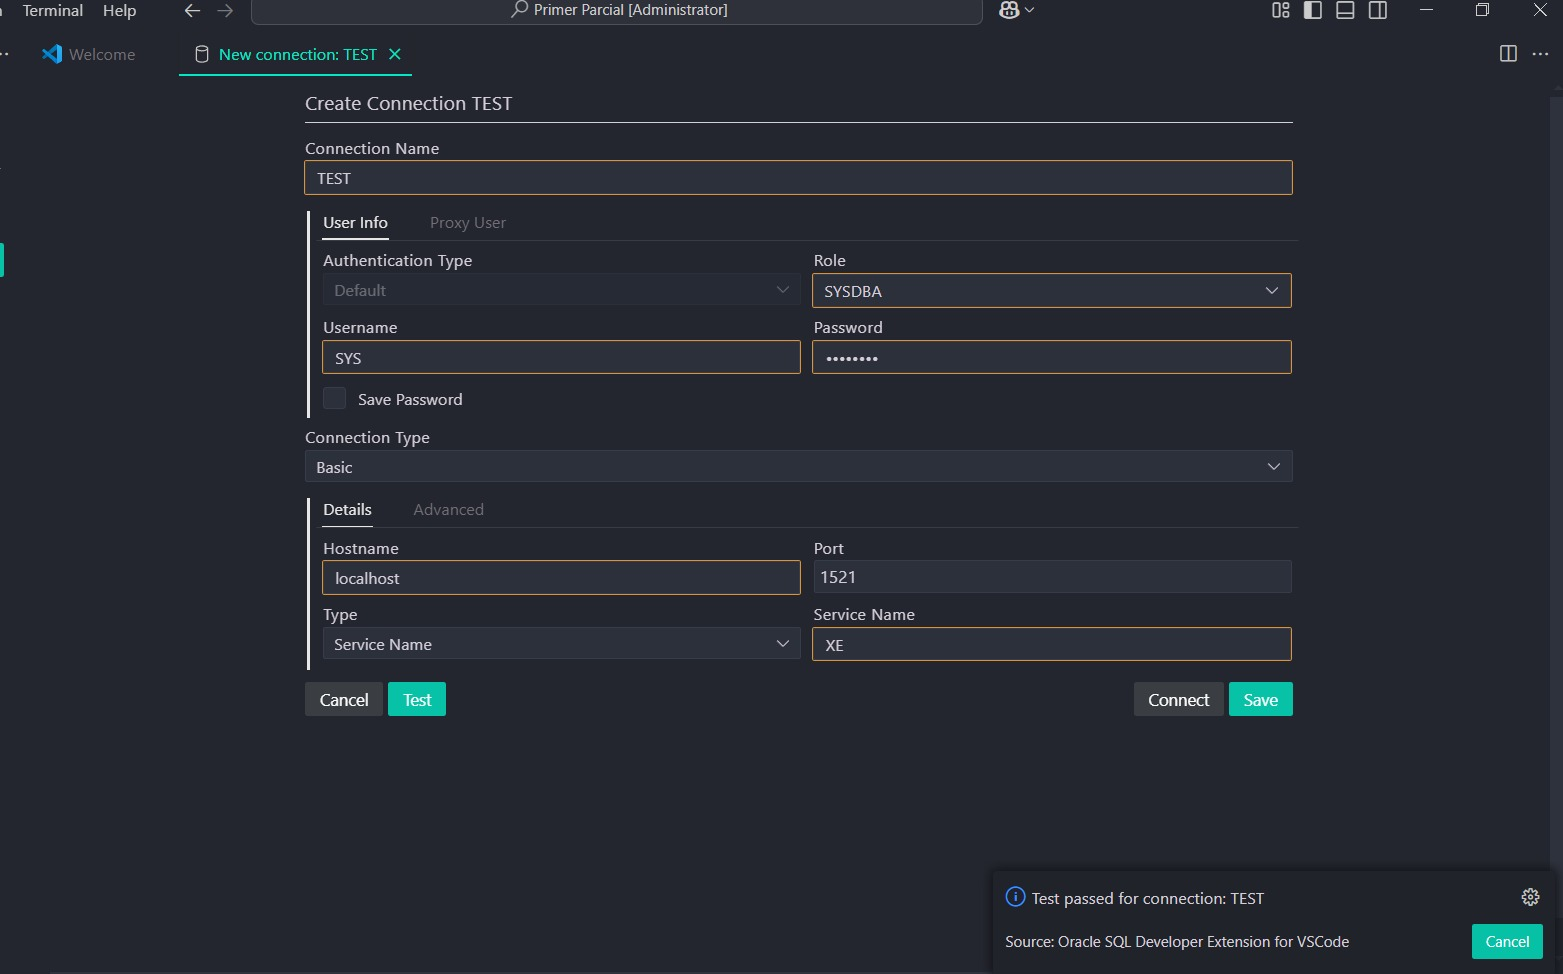
\includegraphics[width=1\textwidth]{imgs/setConn2.jpeg}
	\caption{Setting connection}
	\label{fig:4}
\end{figure}

\begin{figure}[H]
	\centering
	
\includegraphics[width=1\textwidth]{imgs/selConn.jpeg}
	\caption{Connection selection}
	\label{fig:5}
\end{figure}

\begin{figure}[H]
	\centering
	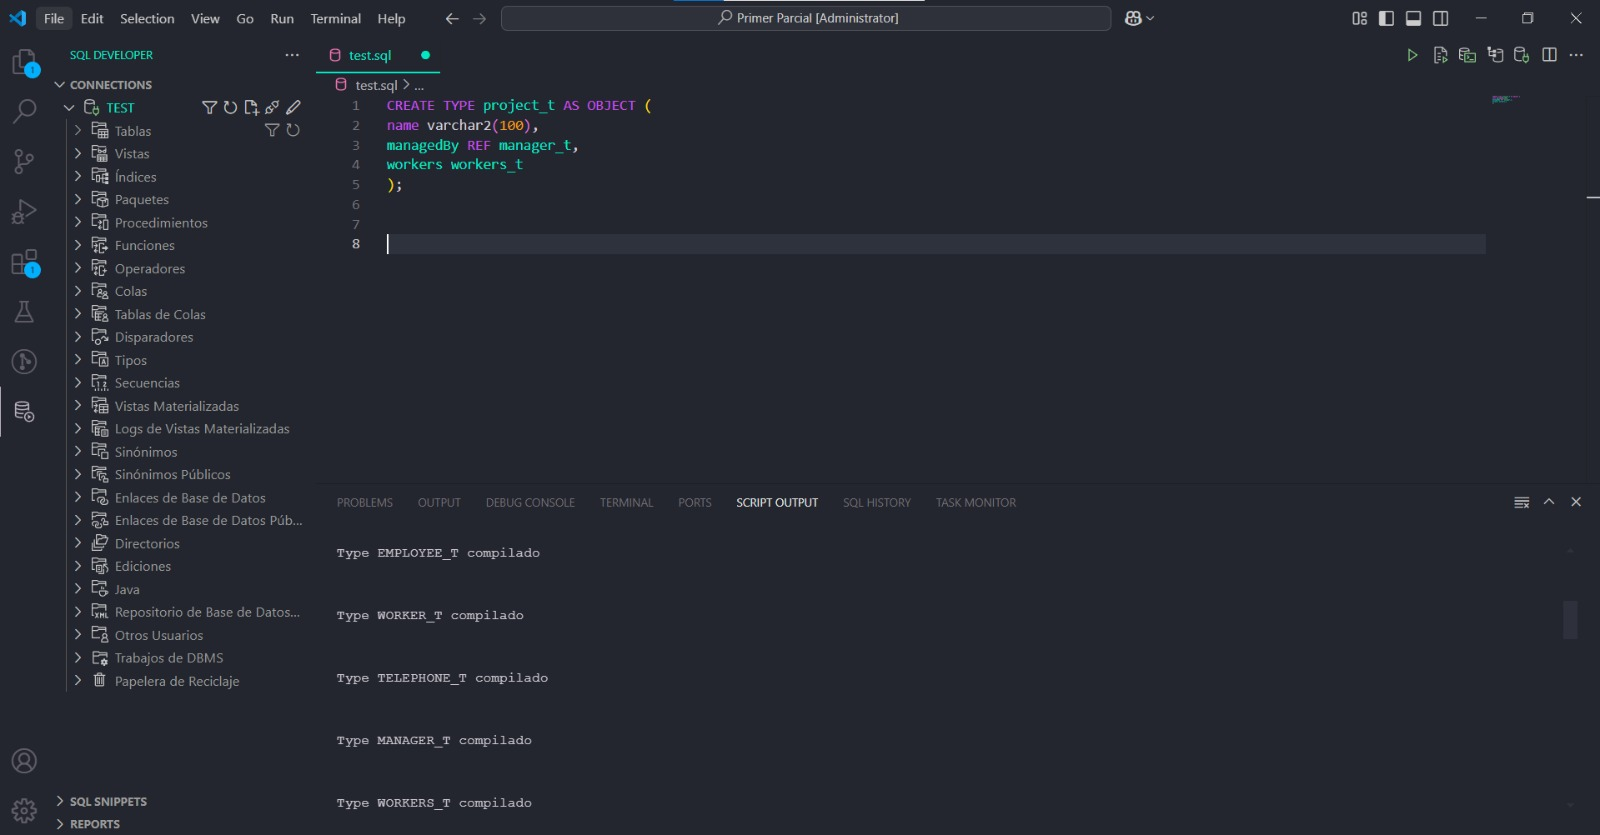
\includegraphics[width=1\textwidth]{imgs/c1.jpeg}
	\caption{Create query}
	\label{fig:6}
\end{figure}

\begin{figure}[H]
	\centering
	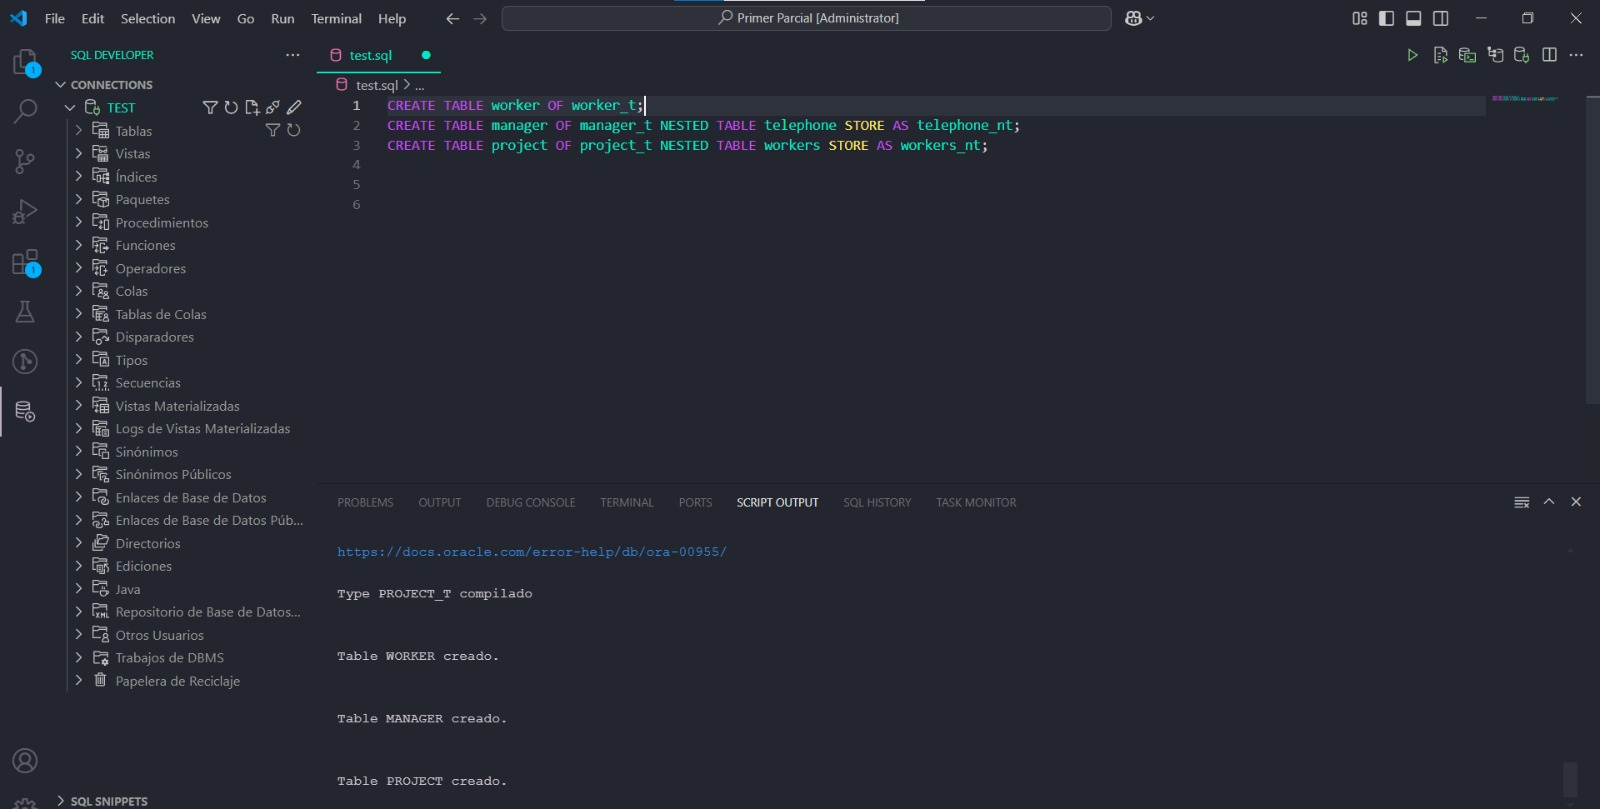
\includegraphics[width=1\textwidth]{imgs/c2.jpeg}
	\caption{Create query}
	\label{fig:7}
\end{figure}

\begin{figure}[H]
	\centering
	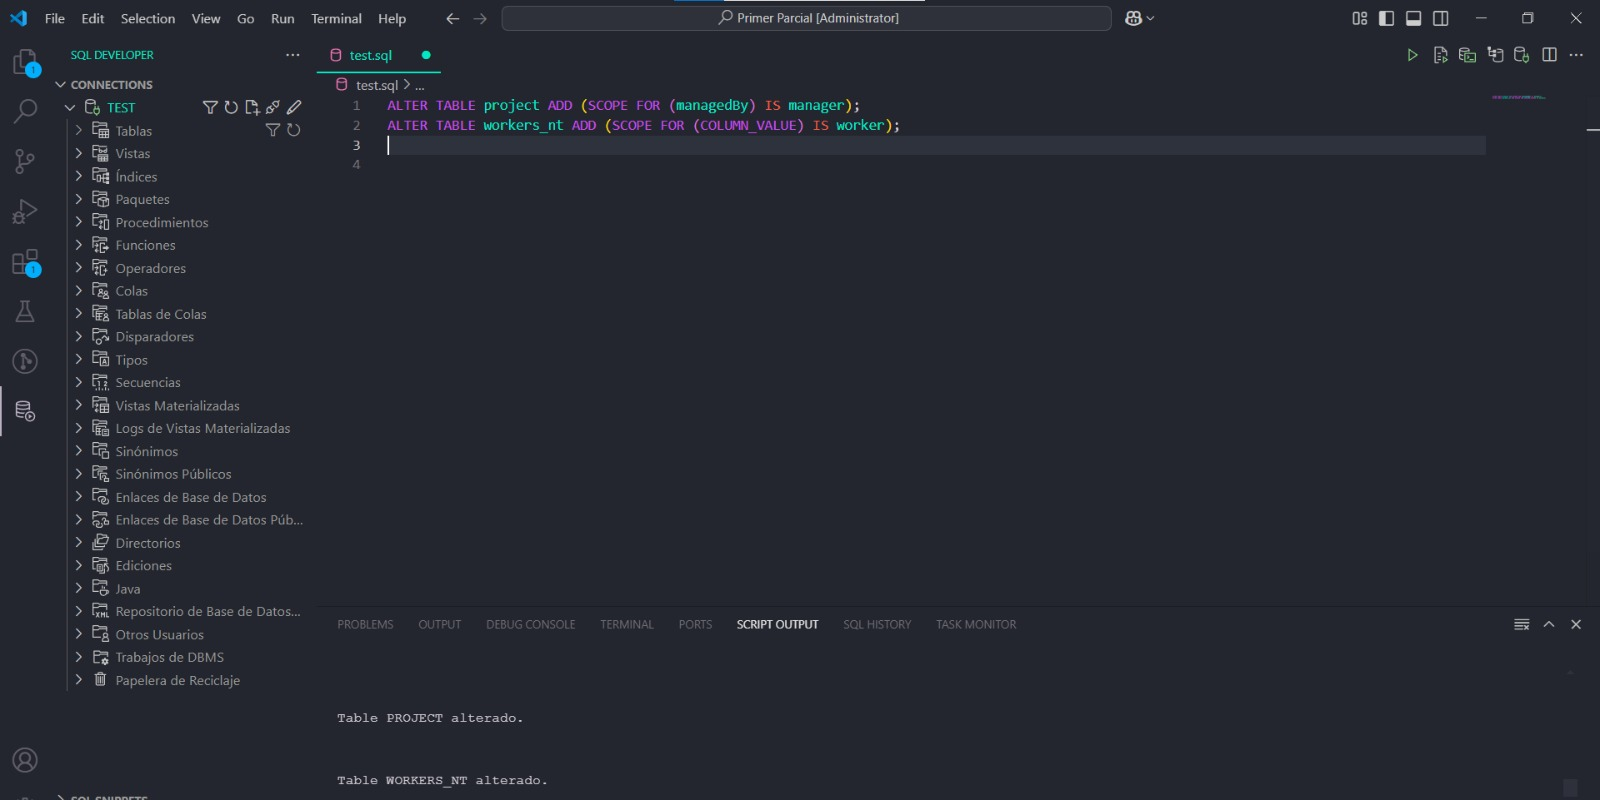
\includegraphics[width=1\textwidth]{imgs/al.jpeg}
	\caption{Alter query}
	\label{fig:8}
\end{figure}

\begin{figure}[H]
	\centering
	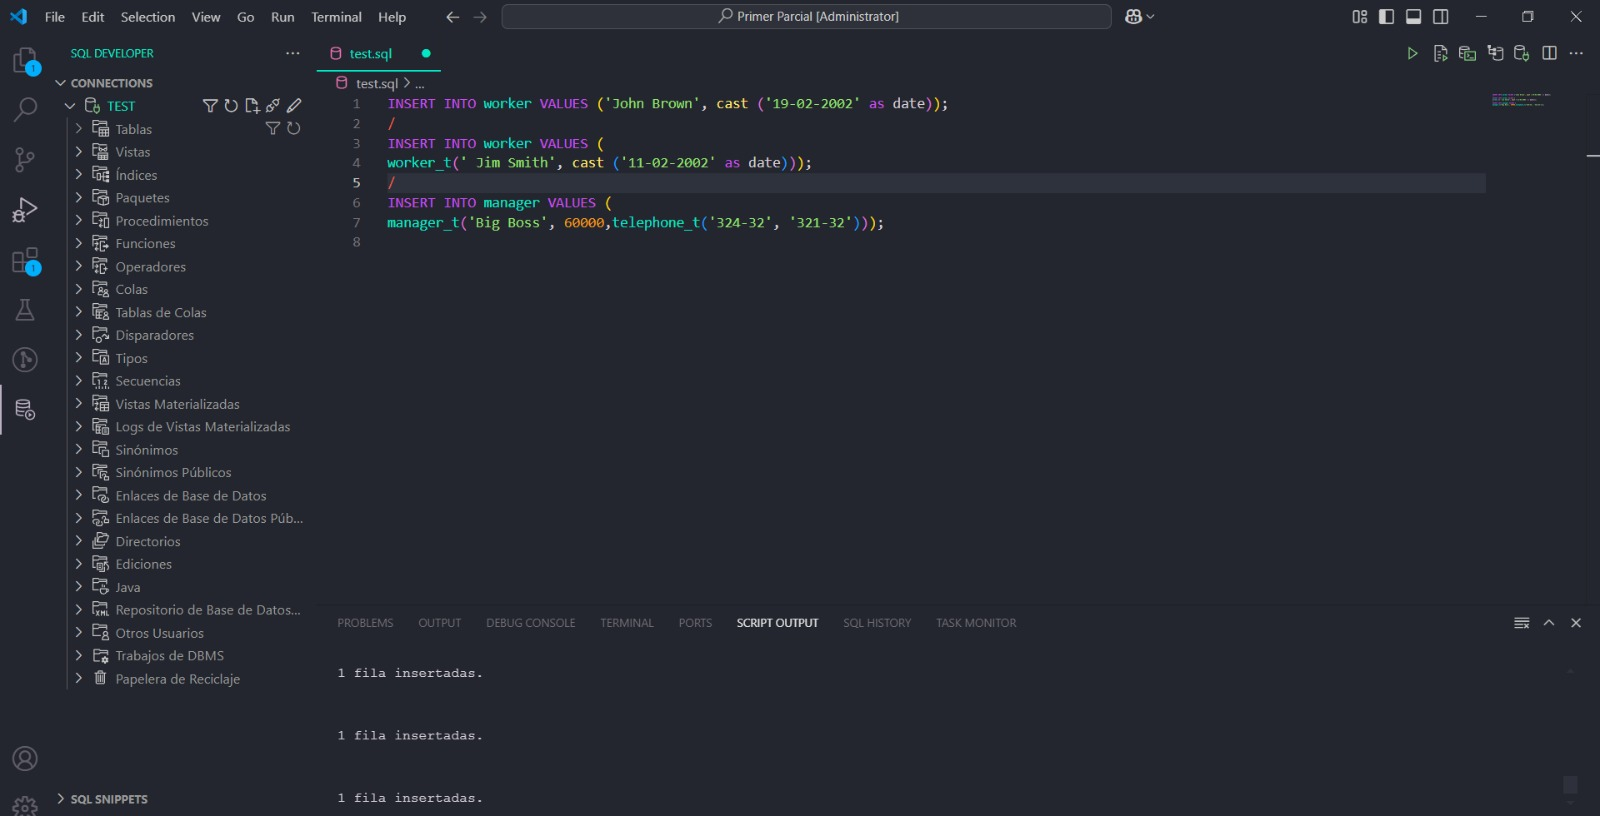
\includegraphics[width=1\textwidth]{imgs/inse1.jpeg}
	\caption{Insert query}
	\label{fig:9}
\end{figure}

\begin{figure}[H]
	\centering
	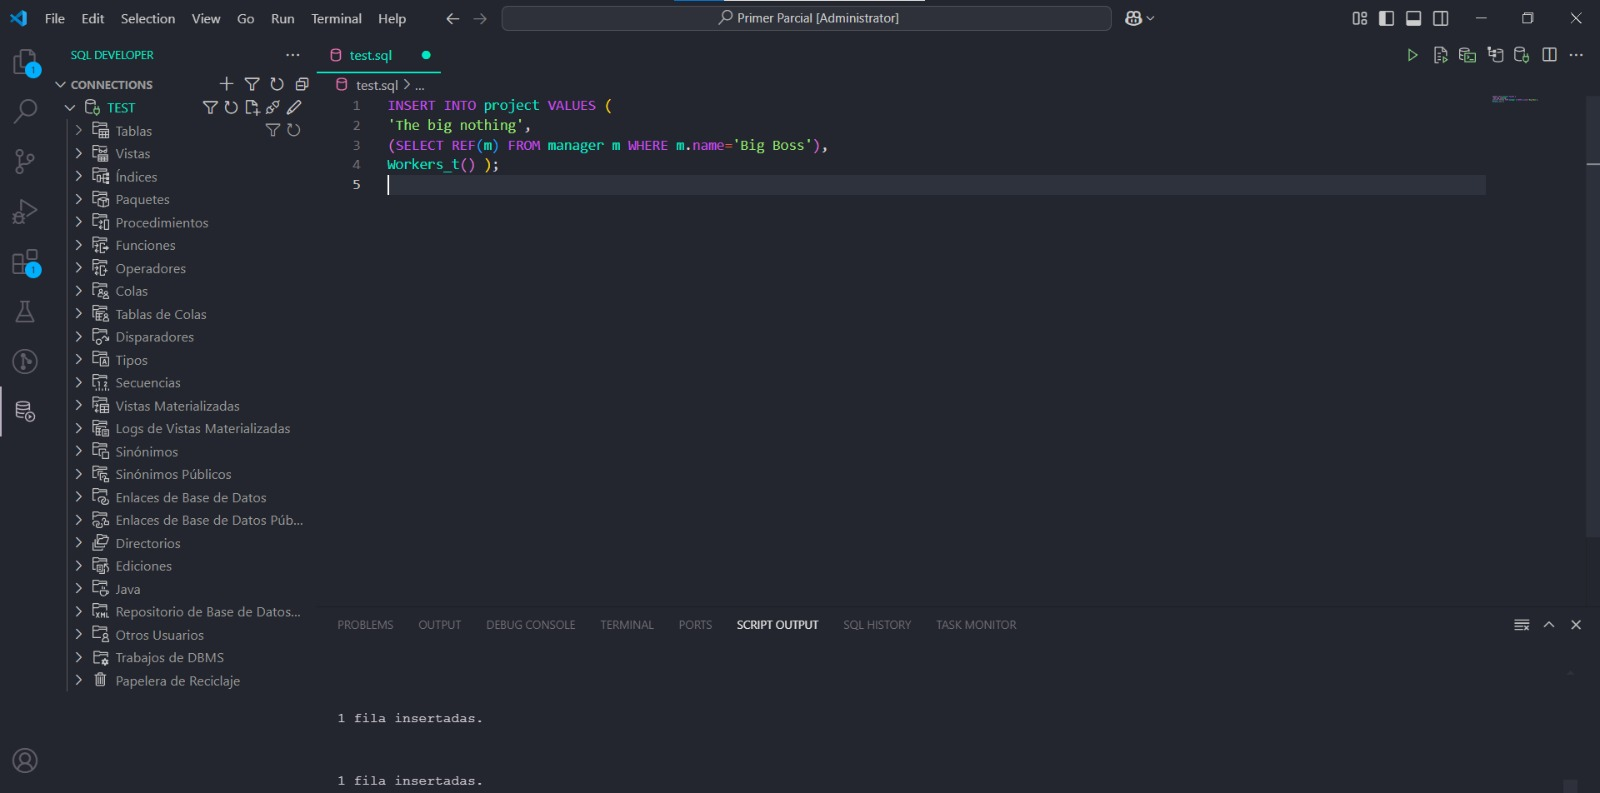
\includegraphics[width=1\textwidth]{imgs/inse2.jpeg}
	\caption{Insert query}
	\label{fig:10}
\end{figure}

\begin{figure}[H]
	\centering
	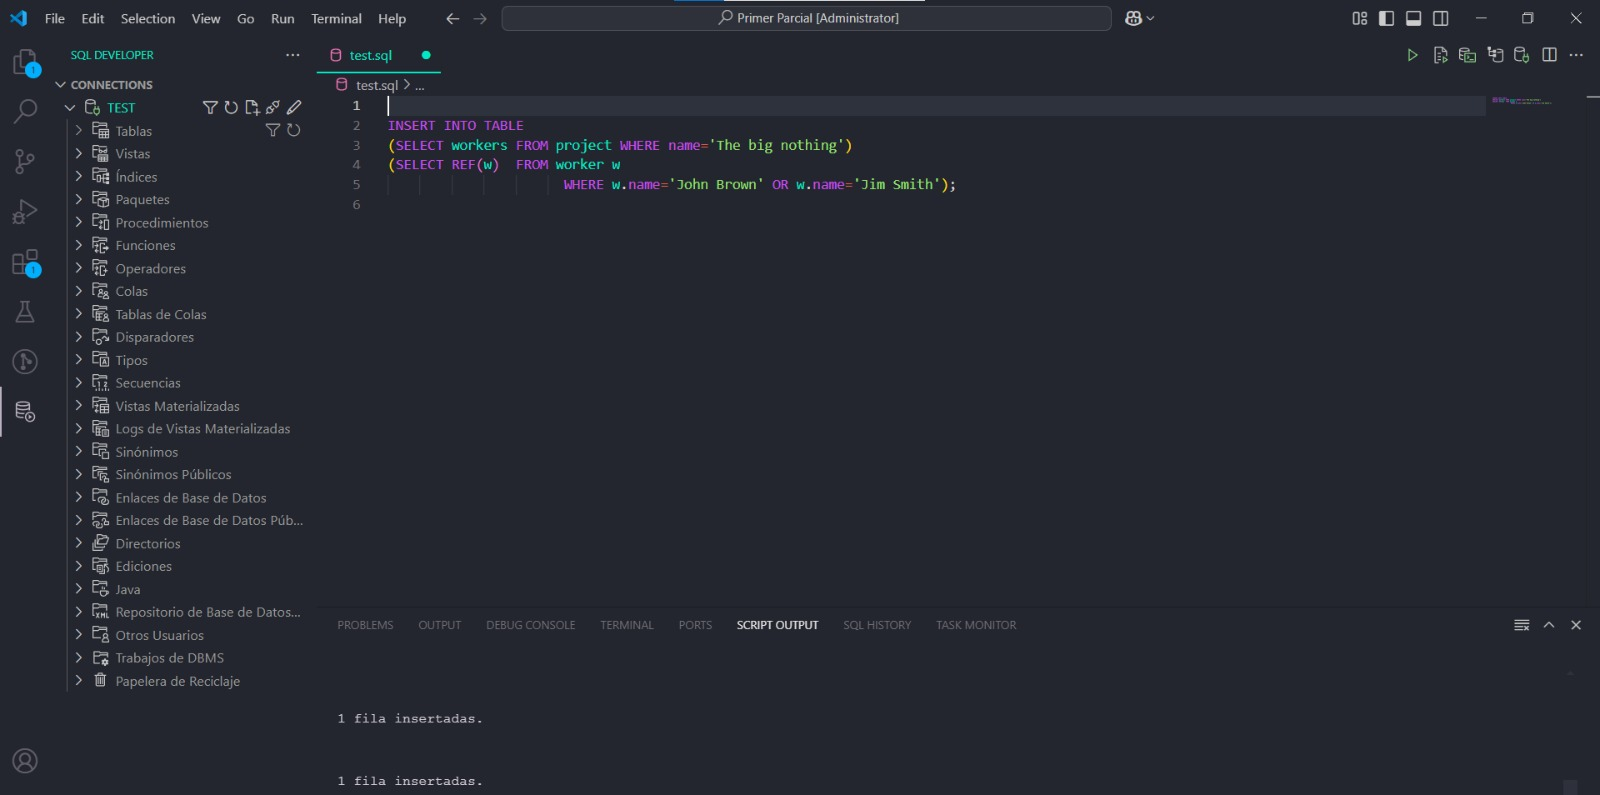
\includegraphics[width=1\textwidth]{imgs/inse3.jpeg}
	\caption{Insert query}
	\label{fig:11}
\end{figure}

\begin{figure}[H]
	\centering
	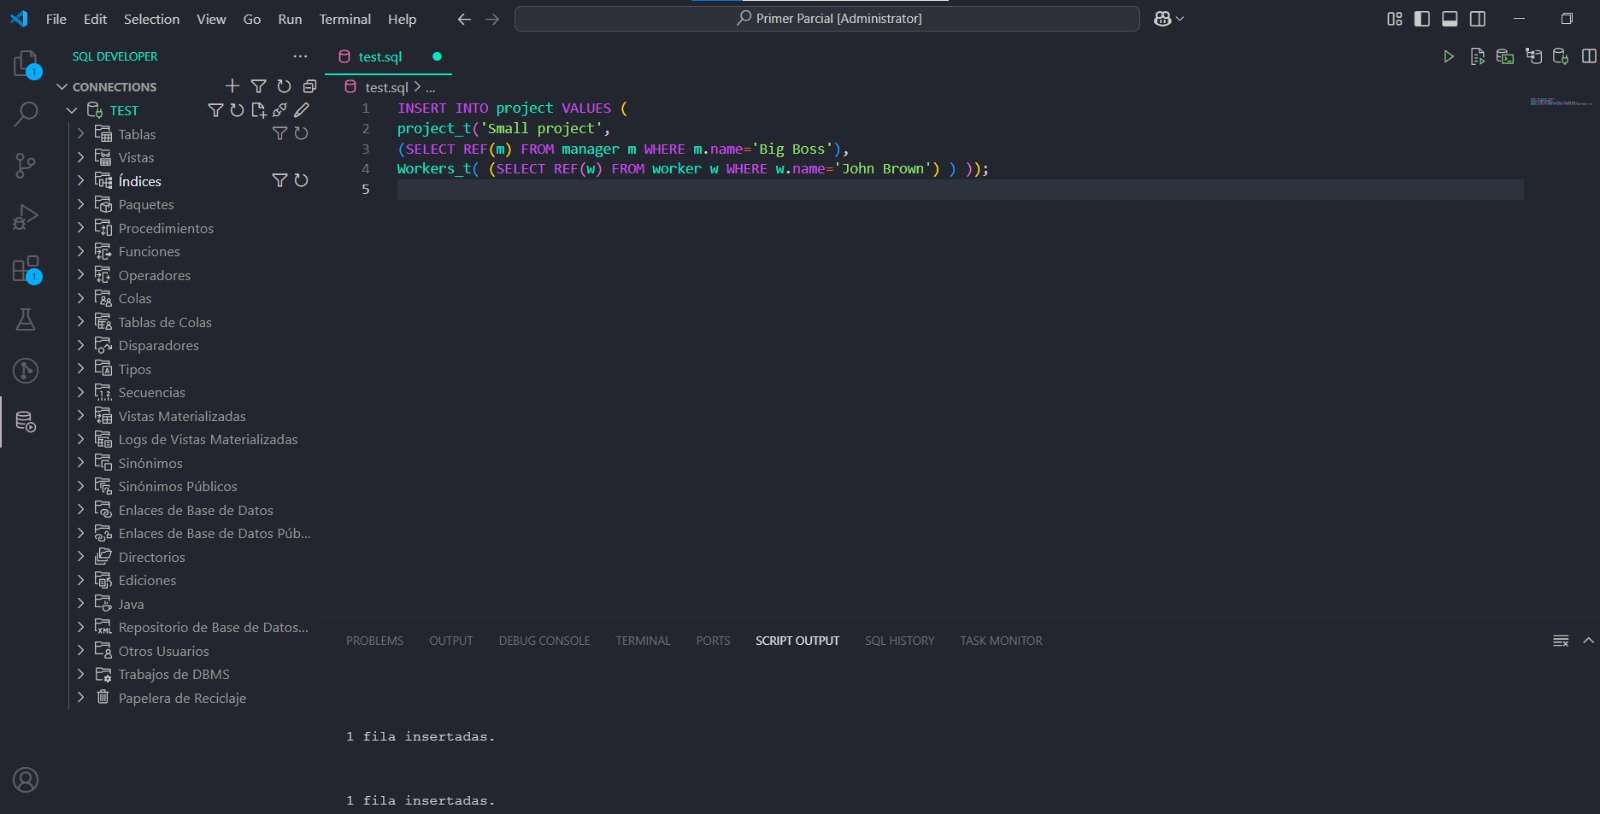
\includegraphics[width=1\textwidth]{imgs/inse4.jpeg}
	\caption{Insert query}
	\label{fig:12}
\end{figure}

\begin{figure}[H]
	\centering
	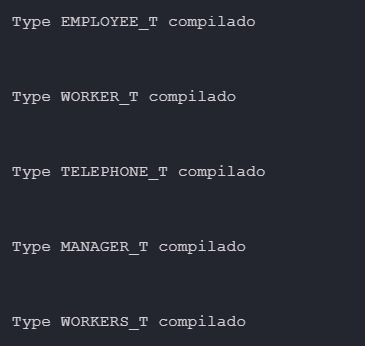
\includegraphics[width=1\textwidth]{imgs/comp.jpeg}
	\caption{compilation successfully}
	\label{fig:13}
\end{figure}


\begin{figure}[H]
	\centering
	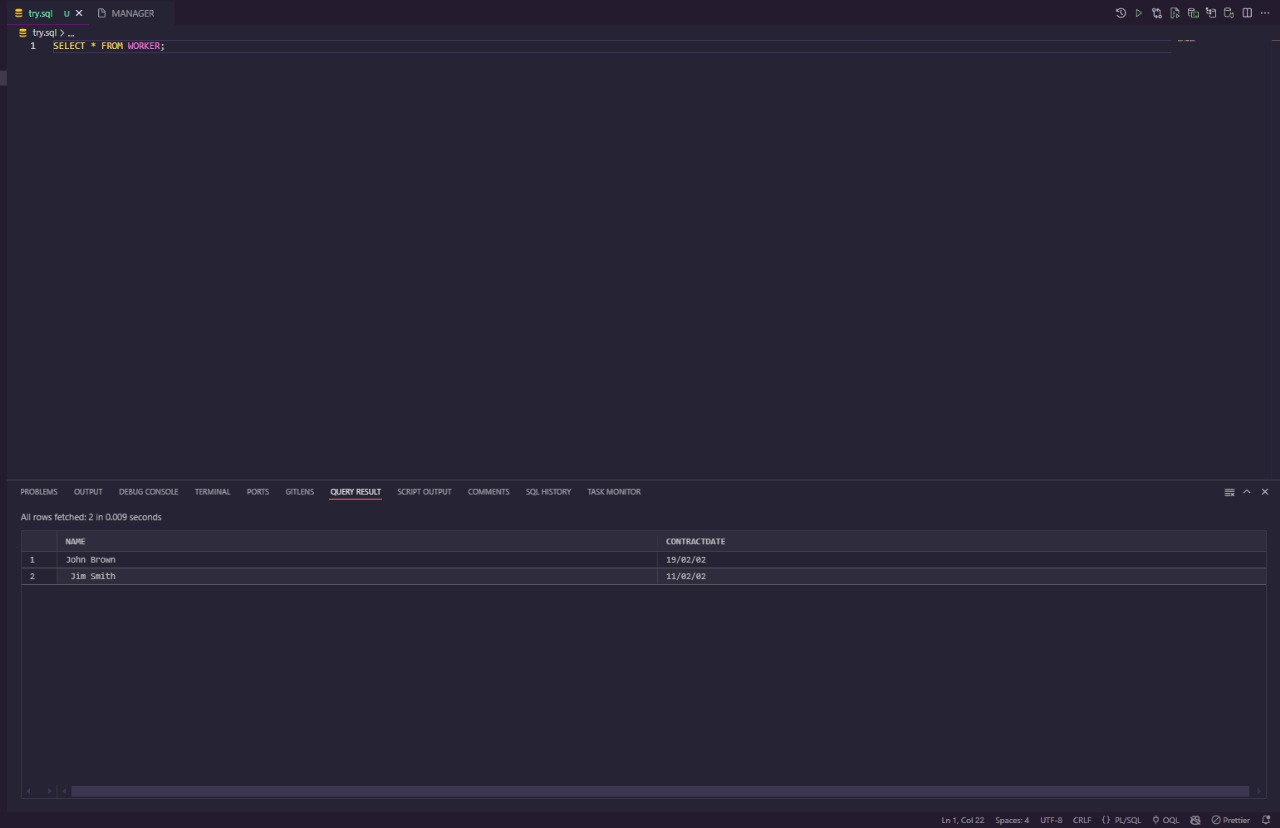
\includegraphics[width=1\textwidth]{imgs/sel1.jpeg}
	\caption{Select query}
	\label{fig:14}
\end{figure}

\begin{figure}[H]
	\centering
	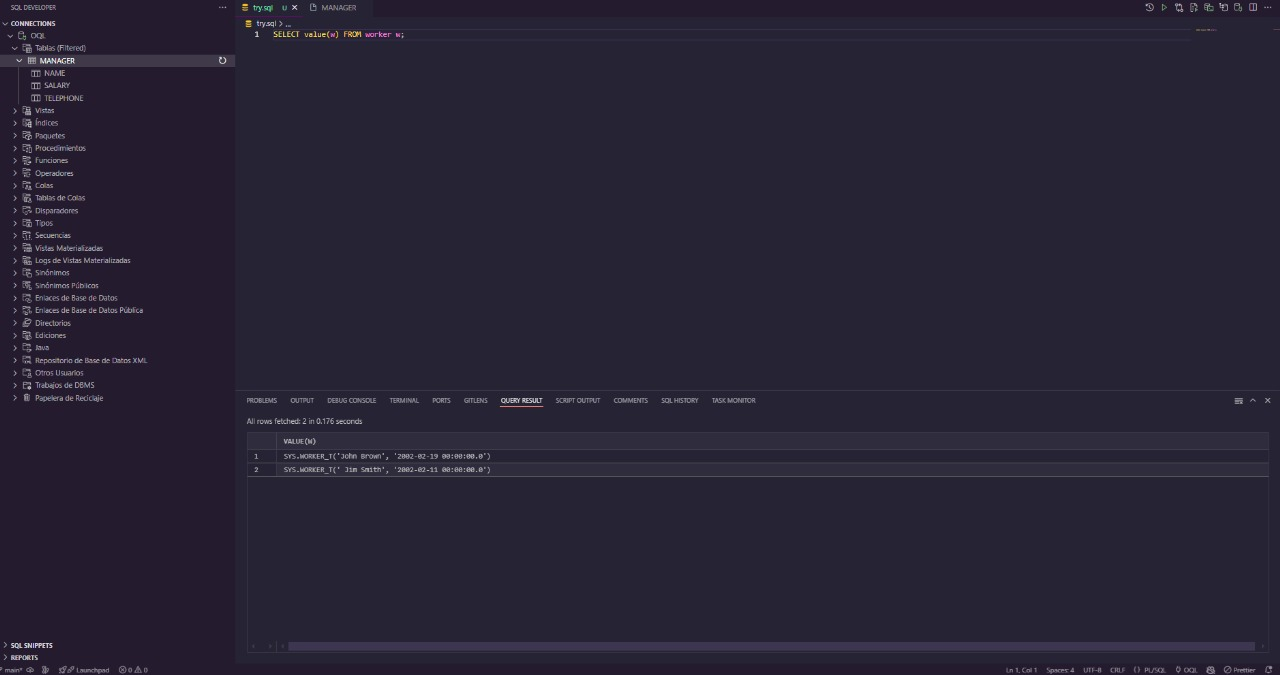
\includegraphics[width=1\textwidth]{imgs/sel2.jpeg}
	\caption{Select query}
	\label{fig:15}
\end{figure}

\begin{figure}[H]
	\centering
	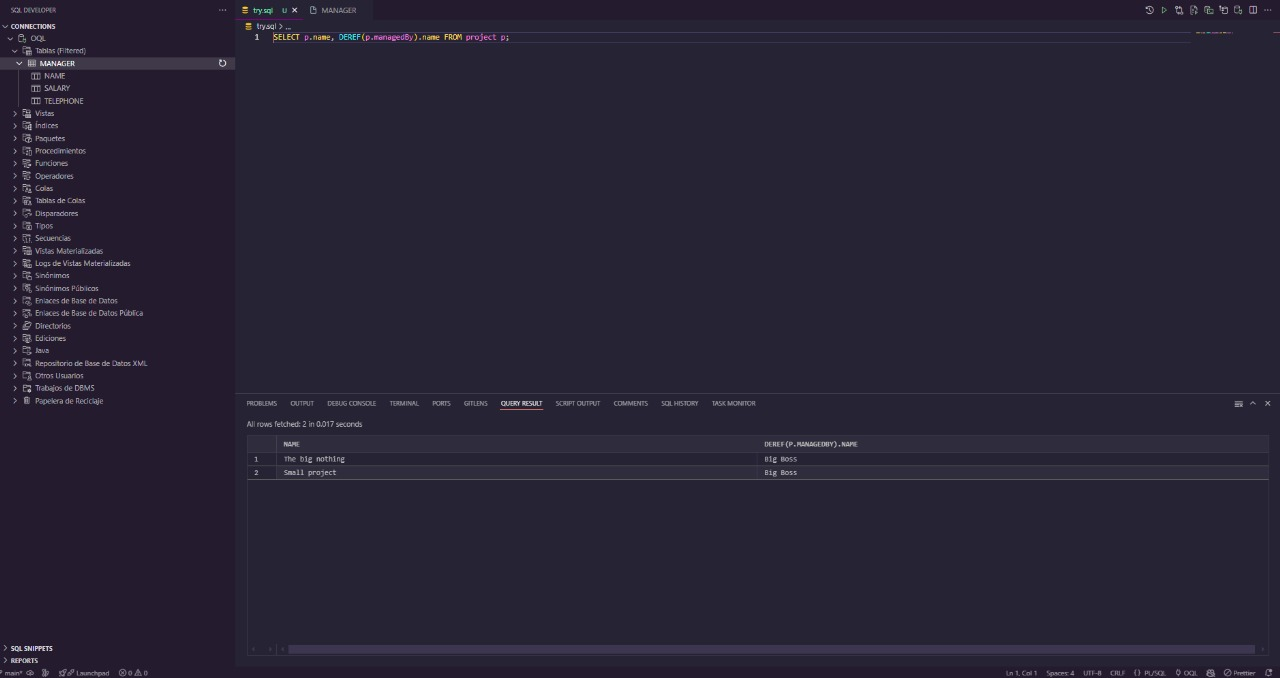
\includegraphics[width=1\textwidth]{imgs/sel3.jpeg}
	\caption{Select query}
	\label{fig:16}
\end{figure}

\begin{figure}[H]
	\centering
	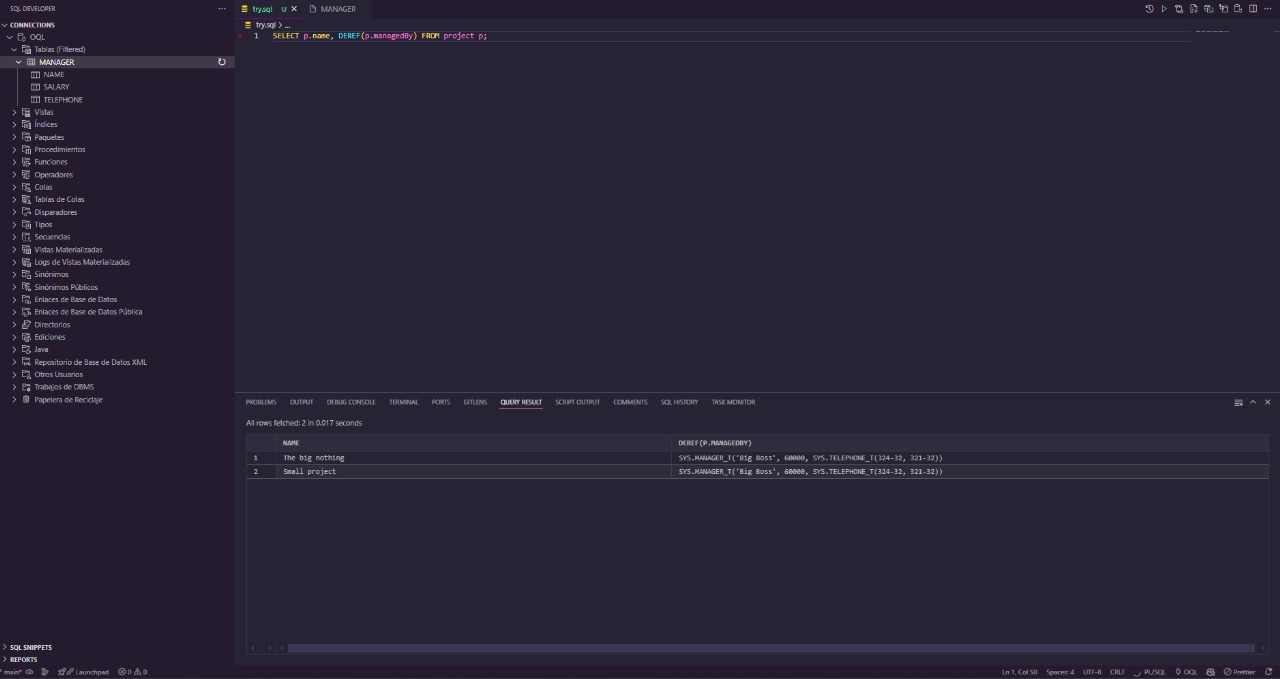
\includegraphics[width=1\textwidth]{imgs/sel4.jpeg}
	\caption{Select query}
	\label{fig:17}
\end{figure}

\begin{figure}[H]
	\centering
	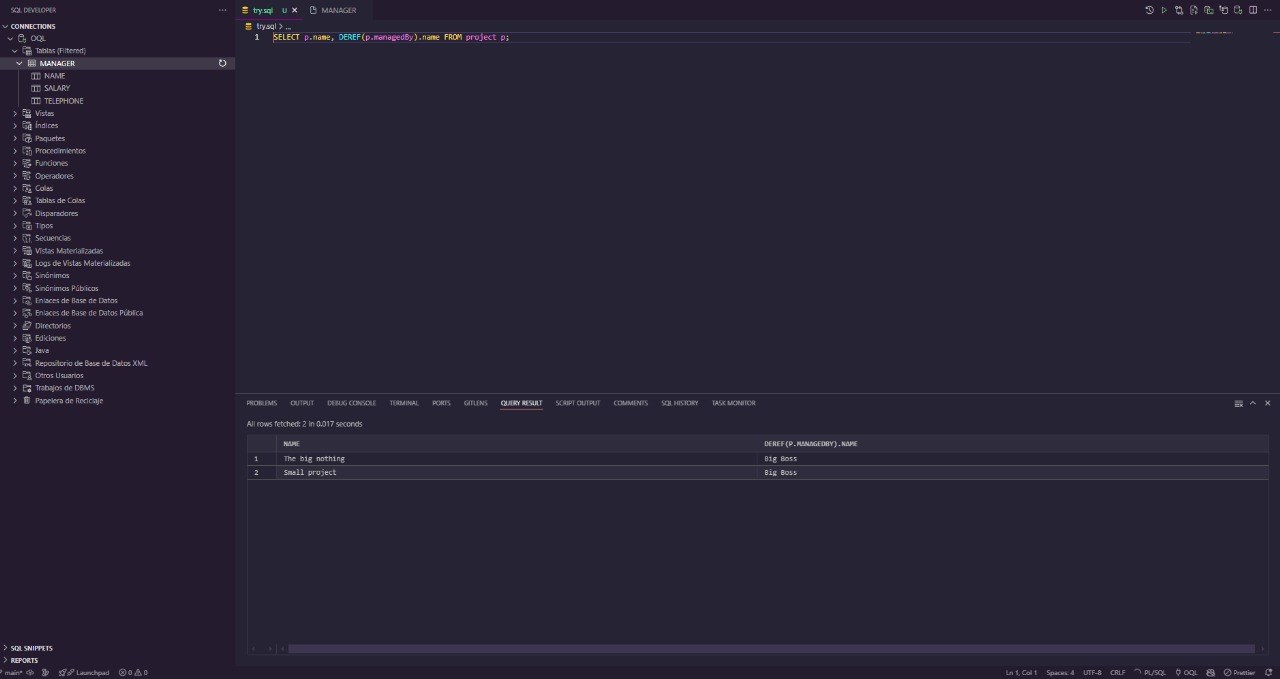
\includegraphics[width=1\textwidth]{imgs/sel5.jpeg}
	\caption{Select query}
	\label{fig:18}
\end{figure}

\begin{figure}[H]
	\centering
	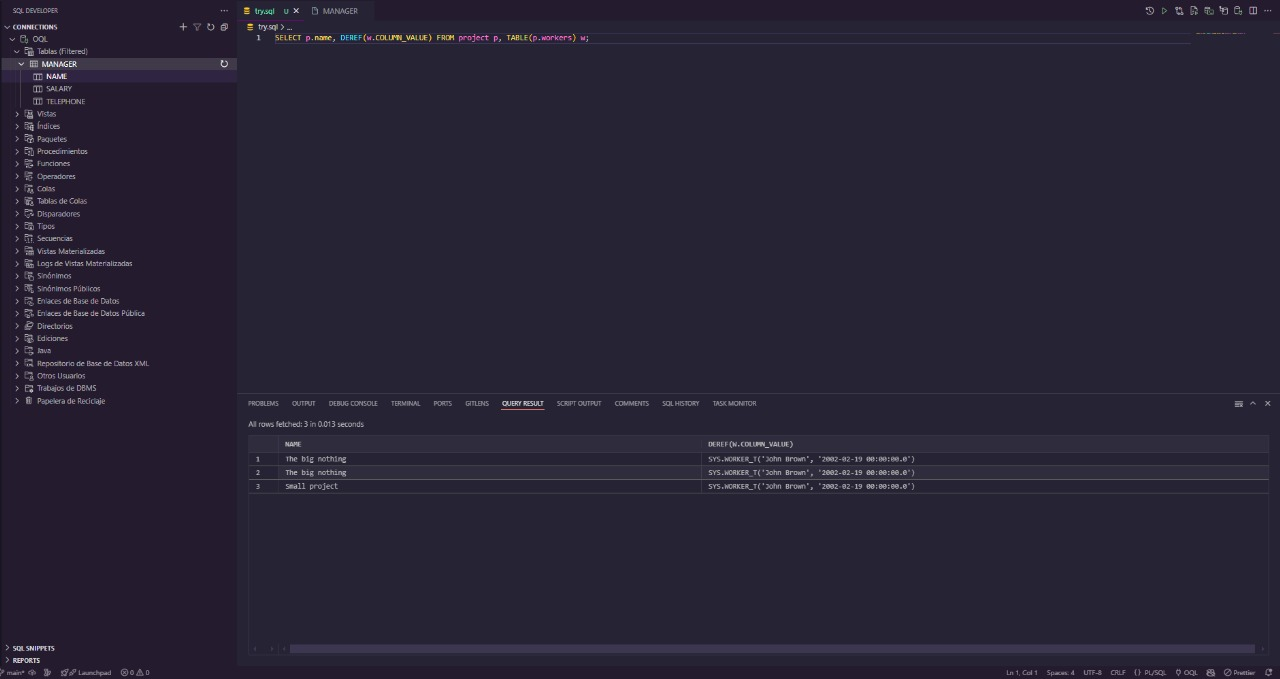
\includegraphics[width=1\textwidth]{imgs/sel6.jpeg}
	\caption{Select query}
	\label{fig:19}
\end{figure}









\section{Conclusions}
This work demonstrated the effectiveness of Object Query Language (OQL) in managing object-relational databases. \textbf{However we as a team struggled a ton to get this tools working due to the lack of documentation that is online.} By defining complex object types, nested collections, and relationships, we showed that OQL simplifies querying object-oriented data compared to SQL, which relies on complex joins. OQL's native support for object-oriented principles, such as inheritance and polymorphism, makes it a superior choice for modern applications. This highlights OQL's potential for advancing database technologies in object-oriented contexts.
\section{EXTRA}
\begin{thebibliography}{9}
	\bibitem{mendix}
	OQL. (n.d.). Mendix Documentation. Retrieved February 7, 2025, from https://docs.mendix.com/refguide/oql/
	\bibitem{ibm}
	Tivoli Network Manager IP edition 4.2.0. (2025, January 21). Ibm.com. https://www.ibm.com/docs/en/networkmanager/4.2.0?topic=reference-object-query-language
	\bibitem{w3s}
	What is SQL. (n.d.). W3schools.com. Retrieved February 7, 2025, from https://www.w3schools.com/whatis/whatis\_sql.asp
\end{thebibliography}

\end{document}
